\chapter{Experimental Procedures}

\section{(6,5) Carbon Nanotube Sample Properties}

\subsection{Sample Preparation}
The sample preparation procedure is well described by Ref \cite{ichinose2017extraction}. For preparing a high-purity (6,5) sample, the process starts with obtaining a CoMoCat solution (Sigma-Aldrich) containing several different chiralities of carbon nanotubes. Gel chromatography is then performed on this mixture to isolate a solution containing a high concentration of (6,5) nanotubes. In this process, the presence of a small concentration (4\%) of sodium deoxycholate (DOC), a surfactant, in the solution prevents nanotubes from clumping together to form bundles. Finally, the sample is pipetted into a quartz cuvette with an optical path length of 1 mm. 

%Include figure of absorption spectrum
\subsection{Sample Absorbance Spectrum}

Measuring the absorbance of prepared samples provides a means of determining the different chiralities present in the sample as well as their relative populations. Here, absorbance $A$ is defined as 

\begin{equation}
A = \log_{10}\left(\dfrac{I_{ref}}{I_{sample}}\right),
\end{equation}

where $I_{ref}$ and $I_{sample}$ represent the optical transmission through a reference sample and the nanotube sample respectively. The reference sample only contains water and a 4\% concentration of DOC and is also stored in a cuvette with an optical path length of 1 mm. 

Figure \ref{fig:sample_absorbance} presents the absorbance spectrum of the (6,5) sample measured using the white-light supercontinuum source described in section \ref{section:white_light_probe}. The spectrum exhibits a number of optical transitions including the $E_{11}$, phonon sideband, $E_{12}$, and $E_{22}$ resonances at photon energies of 1.26, 1.45, 1.9, and 2.17 eV respectively. Furthrmore, other small peaks in the sample at 1.35 and 1.41 eV emerge from exciton resonances of (9,1) and (6,4) nanotubes respectively.

\begin{figure}[H]
	\centering
	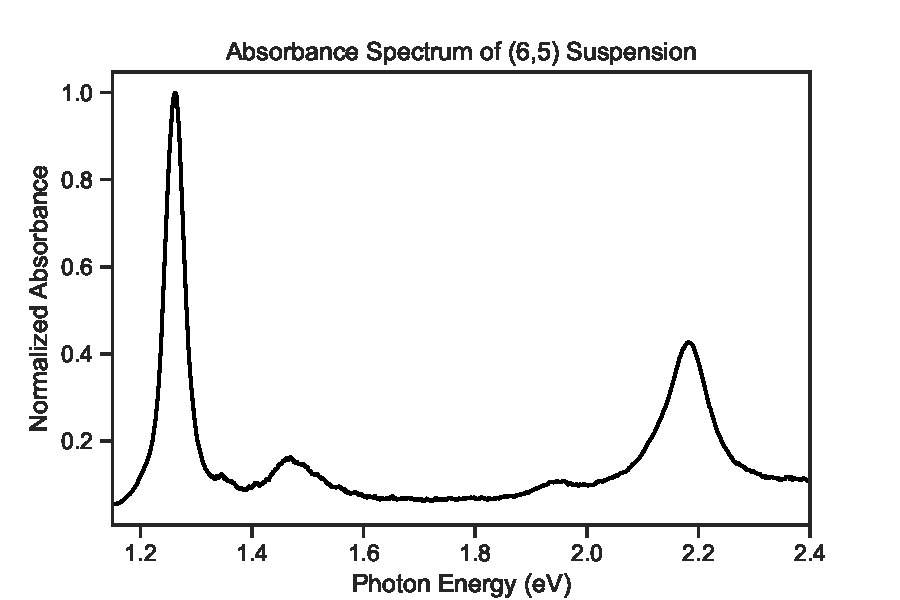
\includegraphics[scale=0.7]{images/chapter_methods/sample_absorbance}
	\caption{ Absorbance spectrum of (6,5) sample.}
	\label{fig:sample_absorbance}
\end{figure}

\section{Experimental Apparatus for Pump-Probe Spectroscopy}

%include figure of setup
\subsection{Overview}
{\color{red} Add a brief summary describing pump-probe spectroscopy and how that is done in this apparatus}. Basic idea of pump probe spectroscopy: two pulses: pump and probe. Pump photoexcites sample. Probe interrogates sample properties. Adjusting the arrival time delay between pump and probe makes it possible to measure dynamics of sample properties with femtosecond resolution. Pump and probe beams are focused onto surface of the sample. Finally, setup is configured such that pump and probe do not travel in a collinear fashion. 


\begin{figure}[h]
	\centering
	\includegraphics[scale=0.7]{example-image-a}
	\caption{ Schematic Diagram of the Experimental Apparatus}
	\label{fig:setup_schematic}
\end{figure}


\subsection{Chirped Pulse Amplifier and Optical Parametric Amplifier}
The CPA-2010 laser source manufactured by Clark-MXR functions as the heart of this optical setup. This laser generates amplified pulses using chirped pulse amplification. It operates at a repetition rate of 1 KHz and outputs pulses with a 150 fs duration and a central wavelength of 775 nm. Finally, the CPA-2010 serves as a pump laser for the optical parametric amplifier (OPA). 

This OPA used in the setup is a TOPAS-800 produced by Light Conversion. It emits signal and idler beams via a superfluoresence in a barium borate (BBO) crystal which are then amplified in four subsequent stages. The signal and idler wavelengths span 1.1 - 1.5 $\mu$m  and 1.5 - 2.7 $\mu$m respectively. Furthermore, an additional BBO crystal placed at the output of the OPA provides a means of generating the second harmonic of the signal which is used as the optical pump beam.

\subsection{Filters}

The setup features a wavelength separator that seperates the fundamental of the signal (FS) from the second harmonic of the signal (SHS). This optical device contains a set of two dichroic mirrors that reflect the SHS and transmit the FS. As a result of the second harmonic generation process, the polarization of SHS remains perpendicular to that of FS. Hence, a half-wave plate is placed in the optical path of the SHS and appropriately adjusted to make the polarizations of FS and SHS parallel to each other. 
 
\subsection{White Light Continuum Probe}


\label{section:white_light_probe}
\textbf{\color{red}UNFINISHED} Supercontinuum generation represents a nonlinear optical process by which the spectrum of an incident laser pulse becomes significantly broadened \cite{dubietis2017ultrafast}. Facilitated by the formation of a filament which starts as a result of self-focusing \cite{dubietis2017ultrafast}. In other words, refractive index of supercontinuum generation medium depends on intensity of propagating light \cite{dubietis2017ultrafast}. Due to interplay between this self-focusing and other effects such as self-phase modulation, and multiphoton absorption, the spectrum spectrally broadens as pulse travels through material \cite{dubietis2017ultrafast}. 

In this setup, supercontinuum generation occurs by focusing the FS into a sapphire crystal which generates white-light continuum that spans 1 - 2.4 eV. Here, a center of a sapphire crystal placed at a distance of one focal length of this lens. Iris used to partially crop the input beam to improve stability of white light spectrum. 

\subsection{Motorized Delay Stage and Optical Shutter}

\textbf{\color{red}UNFINISHED} Setup is equipped with motorized delay stage and an optical shutter which are used to change two key conditions in a pump-probe experiment: time-delay between pump and probe, as well as whether pump is photoexciting sample or not. 

Motorized delay stage changes optical path length traveled by pump. A pair retroreflecting mirrors mounted on a motorized stage is used to adjust optical path length of pump beam which effectively alters timed delay between pump and probe. 

Optical shutter placed in the optical path traveled by the pump beam. At each time delay, measure transmission of the probe beam with the pump beam blocked and with the pump beam unblocked by the shutter.  



\subsection{Spectrometer}
\textbf{\color{red}UNFINISHED}
The probe is collected into an optical fibre which sends this beam to a spectrometer equipped with a charge-coupled device (CCD) camera. Camera is silicon-based and contains an array of 1340 $\times$ 100 pixels. Camera allows to measure the intensity of several wavelengths of probe beam simultaneously. CCD camera is cooled to -100 degrees C using liquid nitrogen for optimal signal-to-noise ratio. 

\subsection{Pump and Probe Spot Sizes}
\textbf{\color{red}UNFINISHED}
Pump and probe spot sizes measured using a knife edge scan. For this, mounted a razor blade on a delay stage placed in the sample position. Measure transmitted power as a function of delay stage positioning. Average power drops as razor blade cuts into beam diameter. This method effectively measures the cumulative distribution function of the incoming beam as a function of the razor blade position.

Assuming that the beam diameter can be approximated as a Gaussian distribution, we can compute the spot size by fitting this data with the equation 

\begin{equation}
	P = P_0 + P_{max}/2 \left( 1 - \mathrm{erf} \left( \dfrac{\sqrt{2}(x - x_0)}{w} \right) \right),
\end{equation}

which represents the cumulative distribution function of a Gaussian distribution. This fitting function yields the beam diameter $w$. Furthermore, $P_0$ represents the baseline of the power meter observed when the beam is fully blocked, erf is the standard error function, $P_{max}$ is the maximum power of the beam, $x$ is coordinate describing lateral position of the razor blade and $x_0$ represents position of razor blade when the razor blade blocks 50\% of the total power.  



\begin{figure}[h]
	\centering
	\includegraphics[scale=0.7]{example-image-a}
	\caption{Example measurement of beam diameter for pump and probe. Solid lines are fits to the data using function defined in equation}
		\label{fig:beam_diamter_measurement}
\end{figure}



